\section{Results}\label{sec-results}

\subsection{First Expectations}\label{sub-sec-firstexpectations}

The authors hypothesised that pupils would be able to achieve a higher
linguistic level as a result of the unquestionable stimulation provided
by the audiovisual tools, which have been demonstrated to address the
learning needs of students. Additionally, in accordance with the
findings of previous research, it was anticipated that the
children\textquotesingle s level of motivation for the subject would
increase.

Nevertheless, it is reasonable to anticipate certain challenges
associated with the computer skills and linguistic proficiency of the
pupils. With regard to the latter, it is important to recognise that
children are simultaneously acquiring three languages without formal
instruction, which could potentially lead to some difficulties.

\subsection{Results on Acquisition of the Language}\label{sub-sec-resultsonacquisition}

As previously stated, the Montessori Method does not include exams,
therefore it was not feasible to propose a pre-test and post-test
framework to collect quantitative data. Consequently, it is not possible
to provide evidence of language improvement, if any. Nonetheless, it was
possible to anticipate certain improvements in their productions, given
that the children were engaged in activities such as translating,
dubbing and subtitling videos, practising listening comprehension,
pronunciation, writing and speaking.

A further defining feature of Montessori is that children select the
areas of study that they wish to pursue. Thus, this approach presented a
significant challenge for them, as their choices were based on the
scenes they enjoyed, irrespective of the level of L2 proficiency
required. This is the reason why the implementation resulted in
unforeseen language difficulties for the children, which obliged the
teacher to provide linguistic support by scaffolding the language.

Although it was not possible to analyse in detail the language
improvement resulting from the implementation, some common mistakes
committed by the pupils could be identified. These can be divided into
two main groups: those related to written productions and those related
to oral ones. In general, the children committed grammatical mistakes in
order to fit the sentences with the speech, such as the removal of the
subjects or the elision of auxiliary verbs. The errors associated with
oral production were primarily related to the rhythm of the
conversations and the pronunciation, particularly that of the vocalic
phonemes, as the pupils read the words in a literal manner. It is
important to highlight the intricate nature of these phonemes for
speakers of Basque and Spanish. In comparison to English, which has
twelve vocalic sounds, the two languages in question possess only five.
Furthermore, the pace of the original dialogues also affected the
pupils\textquotesingle{} oral productions, necessitating adjustments in
their speaking rate to align with the tempo of the original dialogues.

\subsection{Results of the Questionnaire}\label{sub-sec-resultsofthequestionnaire}

Following the completion of the implementation, pupils completed a
survey about AVT and DAT (see \Cref{annex-01}). Unfortunately, as the teachers
did not compel the pupils to fill it, and children were being prepared
for their incorporation to the formal instruction of the next course
(1st of Secondary Education), only seven children answered to the
questionnaire. The questions addressed their opinions regarding the
utilisation of DAT, the motivation it provides and its potential
integration into future English classes. As the pupils are taught in the
Basque language, and given the inherent complexity of the vocabulary and
the dearth of knowledge about the subject matter, the survey was
developed in Basque. However, for the sake of clarity and accessibility,
the sentences have been translated into English in the title of the
figures.

The initial question (see \Cref{fig-01}) sought to ascertain the
children\textquotesingle s level of enjoyment in the workshop. All of
the participants provided a rating that was above the minimum passing
grade. Four children, representing over half of the sample, rated the
workshop with an 8 or 9, while two children assigned a 6, and one child
a 7. These ratings indicate that the children felt at ease and content.
It is noteworthy that none of the children reached the 10-point mark,
given that they live in a multimodal world surrounded by video and
gaming platforms, which are likely to exert a strong influence on their
preferences. It may be posited that the introduction of this novel
activity, coupled with the necessity to master the utilisation of
internet-based tools, has instilled a sense of unease and lack of
confidence amongst them.
\begin{figure}[!htbp]
    \centering
    \begin{minipage}{.75\textwidth}
    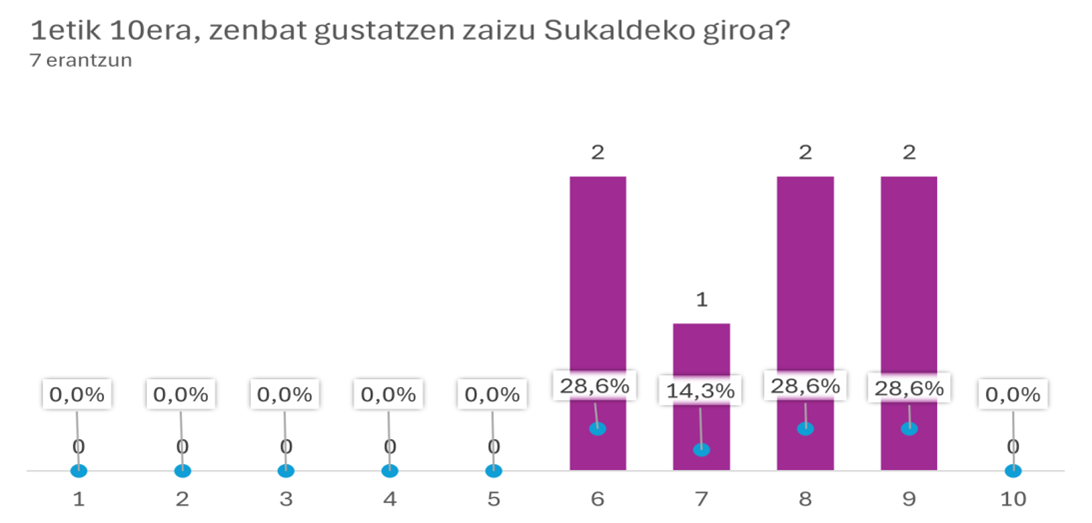
\includegraphics[width=\textwidth]{fig01.png}
    \caption{Question 1. From 1 to 10, how much have you enjoyed
    the ambiance of the workshop?}
    \label{fig-01}
    \source{Owm elaboration.}
    \end{minipage}
\end{figure}

In question 2 (see \Cref{fig-02}), the respondents were asked about their
previous knowledge of AVT. Four of the participants were unaware of its
existence, while the remaining three were cognizant of it. These figures
were unanticipated, given that the children have access to audiovisual
products in three different languages. This may have led them to assume
that there is a process of translation behind that range of options. It
seems reasonable to posit that the most probable reason for this lack of
awareness is that, due to their age, they are accustomed to consuming
audiovisual content in those languages and have not considered the
processes involved.

\begin{figure}[!htbp]
    \centering
    \begin{minipage}{.6\textwidth}
    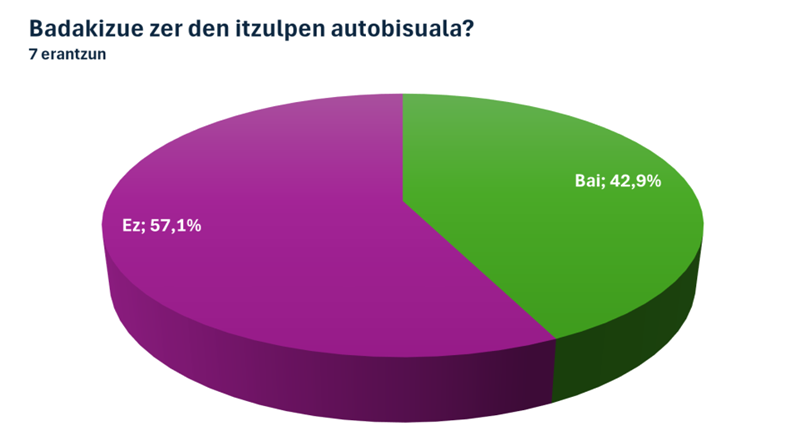
\includegraphics[width=\textwidth]{fig02.png}
    \caption{Question 2. Did you know what audiovisual translation
    was? (green-yes, purple-no).}
    \label{fig-02}
    \source{Owm elaboration.}
    \end{minipage}
\end{figure}

The answers to question 3, if they had enjoyed learning the L2 by means
of the editing of videos (see \Cref{fig-03}) were also positive.
Three-quarters of the children, five, demonstrated a positive attitude
towards the methodology employed, while two of them expressed a negative
opinion. Once more, we may cite the necessity of learning something new
compulsory as the primary reason for their refusal. These results align
with the responses to questions 1, 5 and 6, which will be analysed
subsequently.

\begin{figure}[!htbp]
    \centering
    \begin{minipage}{.6\textwidth}
    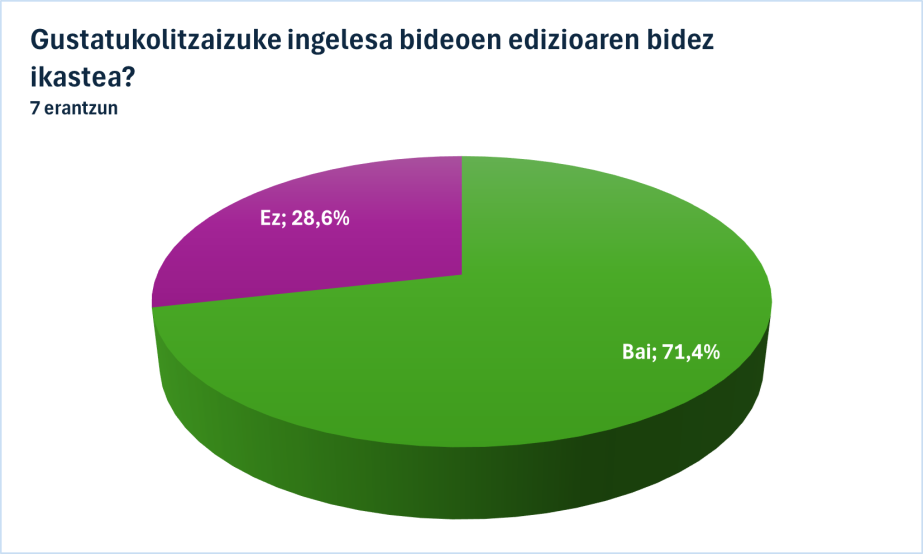
\includegraphics[width=\textwidth]{fig03.png}
    \caption{Question 3. Have you enjoyed learning English by
    means of video editing?}
    \label{fig-03}
    \source{Owm elaboration.}
    \end{minipage}
\end{figure}

In response to question 4, which pertains to the two modes implemented
in class and translation (see \Cref{fig-04}), it can be observed that data do
not provide a clear indication of the pupils\textquotesingle{}
preferences towards either mode. The preference for dubbing is indicated
by a single pupil, while the other two modes were selected by two pupils
each. It is noteworthy that two children selected translation, a written
activity that is not directly relevant to their lived experience, rather
than the other two modes, which are inherently more visual.

\begin{figure}[!htbp]
    \centering
    \begin{minipage}{.6\textwidth}
    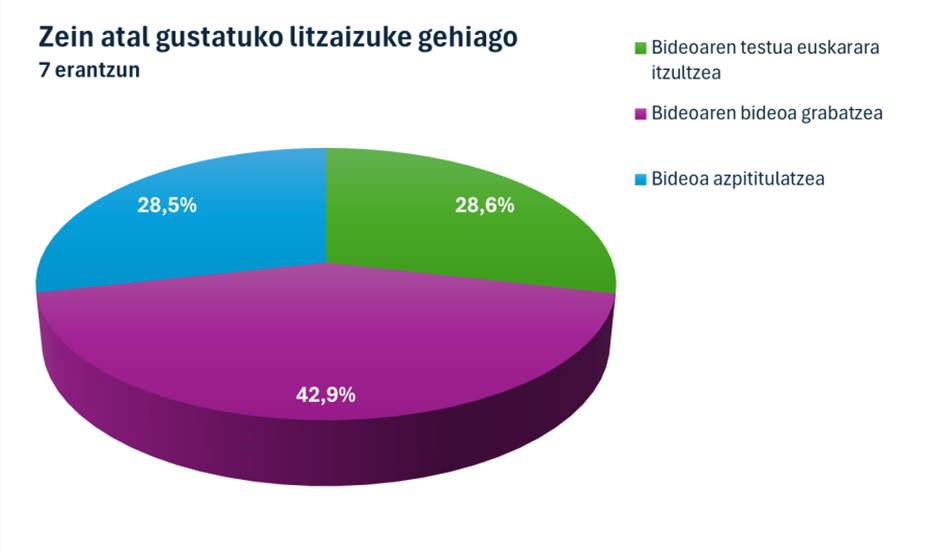
\includegraphics[width=\textwidth]{fig04.png}
    \caption{Question 4. Which tool have you liked the most?
    (Green: interlingual indirect translation of texts; purple: dubbing;
    blue: subtitling).}
    \label{fig-04}
    \source{Owm elaboration.}
    \end{minipage}
\end{figure}


In question 5, the children were asked about the process of language
acquisition. As illustrated in \Cref{fig-05}, all pupils demonstrated an
understanding that they would benefit from these educational
initiatives. It is noteworthy that five of the pupils awarded the
project an 8, a high rating that reflects their trust in DAT. One pupil
considered the quality to be satisfactory, while one rated it slightly
above average. Overall, the marks are deemed satisfactory, as none of
the responses were below the passing mark of 5. These responses are
consistent with those provided in question 2, in which two children
indicated a lack of knowledge regarding AVT.

\begin{figure}[!htbp]
    \centering
    \begin{minipage}{.75\textwidth}
    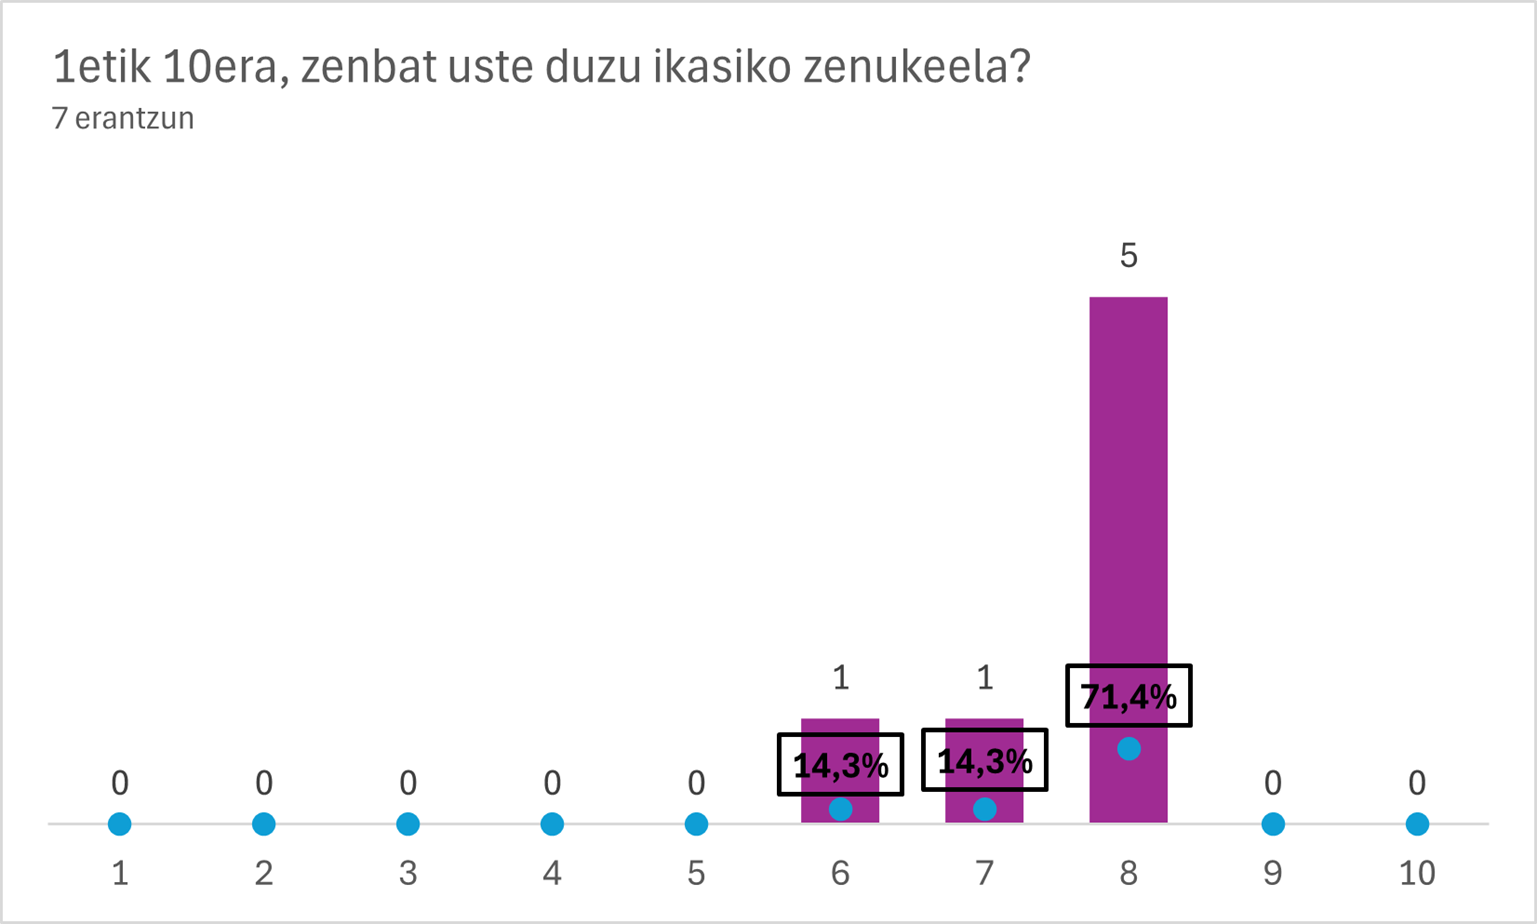
\includegraphics[width=\textwidth]{fig05.png}
    \caption{Question 5. From 1 to 10, how much do you think you
    would learn?}
    \label{fig-05}
    \source{Owm elaboration.}
    \end{minipage}
\end{figure}

The final question (number 6) asked the pupils whether they would
like to engage in DAT activities within the classroom setting. Five
pupils responded in the affirmative, while the remaining two expressed
opposition to the proposal. However, their responses lacked sufficient
clarity or referenced their disapproval of the instructor rather than
the DAT activities themselves. It can be inferred that these two
students are the same individuals who, in question 1, rated the workshop
atmosphere as 6, who provided negative responses to question 3 regarding
their enjoyment along the process, and who rated the development as 6
and 7. This is somewhat surprising, given that these ratings are not
particularly low.

Question 6 (original answers in \Cref{annex-03})

\begin{itemize}
    \item \textbf{Pupil 1}: Yes, because I learn.
    \item \textbf{Pupil 2}: Yes, because I like making videos a lot.
    \item \textbf{Pupil 3}: Yes, because I have never tried it and I think it would be good.
    \item \textbf{Pupil 4}: Yes, because I like recording videos a lot.
    \item \textbf{Pupil 5}: Yes, because it is fun.
    \item \textbf{Pupil 6}: No, because I do not want X (a teacher) to appear.
    \item \textbf{Pupil 7}: No.
\end{itemize}
